\chapter{Introduction}

On the context of this thesis and the motivations that encourage for this work.

\section{Context}
\lettrine{A}{typical} configuration for high performance machines are clusters.
It means a team of individual processors or multiprocessors 
(and lately more specific 
hardware like GPUs) working together, interconnected by a super-fast network. 
The fundamental idea behind these big machines is getting speedup by mean of
partitioning the problem and parallelize the execution. So all processors (or a 
subset) in the cluster will be dealing with different parts of the same problem 
and communicating between them in order to end up with a solution. For example 
imagine we have a weather forecast software, in order to speedup the forecast 
we can partition the surface of the earth and hold every portion to one individual
processor. The communication will be needed because the weather will also depend 
on surroundings, so every partition will need also information of other partitions 
results.

In Computer Science the discipline in charge to drive research in this field is 
the High Performance Computing, i.e. HPC. HPC has been increasing in importance 
and nowadays can be said it is the third support of science with theory and 
mathematics. The science that can be done thanks to this big machines goes from 
earthquake predictions to the analysis of the DNA of a carcinogenic cell, from
weather forecast to material physics simulation. HPC research is not just limited
to the hardware layer but drive research in all layers in the Transformation 
Hierarchy\cite{transformationHierarchy} in figure \ref{transformationHierarchyImg}.

\begin{figure}
  \caption{Levels of transformation}
  \label{transformationHierarchyImg}
  \centering
    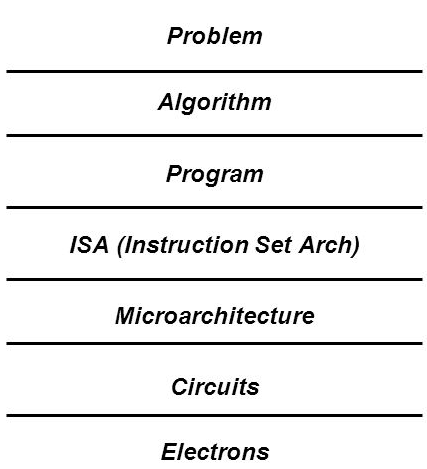
\includegraphics[width=100px]{transformationhierarchy.png}
\end{figure}

Resources are limited and expensive, so we have to be smart and use them in an
efficient way. Improving the efficiency is not just a matter that affects to one
layer of the stack but can be applied to every one of them. For example the
tremendous evolution of the last fourty years were improvements done mostly on
circuits layer what have been following the Moore's law \cite{moore:1965}. The
manufacturers have been reducing the size of transistors by a ration of 2 every
18 months as were predicted in figure \ref{moore-prediction}. Performance improvements 
were also at microarchitecture level with
disruptive designs that allows ILP like HPS\footnote{High Performance Substrace,
what is indeed out-of-order execution with in-order retirement.}
\cite{Patt:1985:HNM:18927.18916}, speculative execution with prefetchers, 
branch prediction or even memory access value speculation,
VLIW\footnote{Very Long Instruction Word} or TLP\footnote{Thread Level
Parallelism} with multi-threading. Improvements on memory hierarchy like cache 
associativity, non-blocking cache or trace cache. The last
big revolution affected both architecture and program layers and was the 
multicore revolution. Was specially important because until then, programmers were 
agnostics, just feel their programs went faster but now, programs have to be 
architecture aware. With this last revolution a new effort for hide machine stuff
from programmers arise and end up with programming models like OpenMP
\cite{openmp_new}, OpenACC\cite{openacc_new} or OmpSs\cite{ompss_new}. A relatively
recent example is shown is this paper \cite{Alvarez:2015:CPT:2872887.2750411}
where they are trying to automatically use the fast scraptchpad memories by
means of compilers procedures and extra hardware support instead
of let programmers to deal with this piece of hardware directly. So be 
always faster and faster is a big deal and is even more pressing in HPC because 
as it is sayd, it is fact an important science driver.

\begin{figure}
  \caption{Gordon Moore's prediction done in 1965}
  \label{moore-prediction}
  \centering
    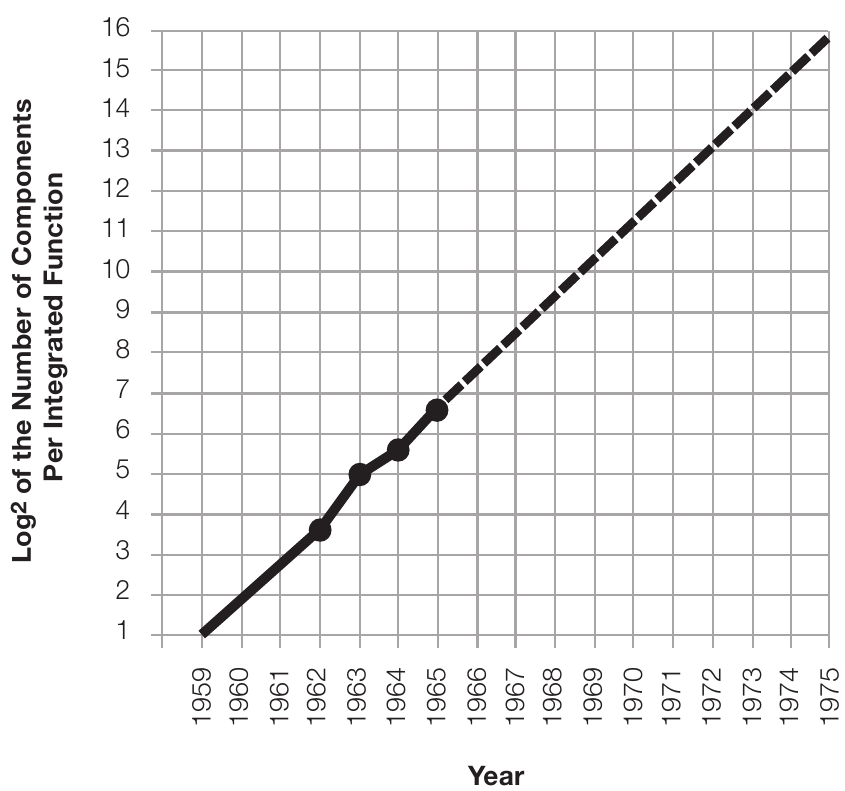
\includegraphics[width=150px]{moore_prediction.png}
\end{figure}


This thesis is centered on program layer\footnote{The program layer 
bring together the program itself, programming models, frameworks and libraries.}. 
This layer is the actual implementation of the algorithm, i.e. where programmers
transforms algorithm to  semantic code that can be transformed lately into
executable binary by compilers. This layer is indeed the interface between pure 
algorithm and the machine architecture. Having an efficient algorithm
mathecamically speaking is not enforcing having an efficient program 
because at algorithm level we do not care about the machine. 
The mechanism to assess the quality in terms of performance are the performance 
analysis tools that allows to analyze and detect the bottlenecks. 
There are two main trends, by one hand we have the profilers and by other hand trace
tools. Profiler tools provide performance summaries. This summaries provides 
coarse-grain information, with low-overhead. It means that you can feel the problem 
and infer what could be the origin but the information is not enough if you want 
to be sure. For gather more detail, the other typical approach are the tracing 
tools. High accurate and detailed information can be obtained, but it needs 
more resources in terms of cpu, disk and analyst effort because more data implies 
more complexity. This demand of resources becomes worst since the capacity in 
terms of parallelism is increasing, so the number of tasks to monitor makes 
tracing by one hand hardly scalable and by the other hand tricky to analyze
because the huge quantity of data and because the increasing response times
during the interactive exploration of analysis results. 

Researchers are currently facing this two drawbacks. There are currently several
specialists driving research in the scalability field, they are trying to reduce 
the overhead of tracing in terms of time and trace sizes by mean of several 
techniques like machine learning, data-mining and so on like in 
\cite{llort2015intelligent} or by on-line compression like in
\cite{noeth2009scalatrace}. About analysis field, the complexity of the analysis 
can be overcome by adding intelligence to performance analysis tools, last 
trend is to provide an automatic smart layer that automate an important part 
of the analysis. Some examples of this 
research line are automatic performance analysis \cite{wolf2003automatic}, 
automatic structure extraction \cite{casas2007automatic}, phases detection 
\cite{gonzalez2013application} fundamental factors models \cite{casas2008aass}, 
automatic analysis throw deep learning \cite{simon:2017:perfdp} and so on.

This thesis is focused on the analysis field and is devoted to humbly contribute 
to ease the work of the analyzers by
automate part of the analysis. The goal of this work is to automatically detect
the internal structure of an application and correlate it with performance metrics by
mean of a post-mortem trace analysis that will help to have a general
overview about what is actually going on. So instead of deal with whole
information from the very beggining, this approach let the analyzer to figure
out to what part of the gathered information focus on, speeding up the process of
analysis. Also will help to correlate performance analysis with source code
since the detected application structure would be similar as
code structure. Furthermore it will contain source code information that will allow to
easly pinpoint one metric to the code. The structure representation will ignore 
implementation details what therefore will contribute to faster and therefore better 
quality reports for developers. 

This sort of analysis have been done tipically by using sequential pattern mining
techniques what is in principle the set of techniques that better fits to this
problem since a trace is just a sequence of events ordered by time. The main
drawback of these techniques is the complexity of the algorithms that behaves
linearly in the best case and exponentially in the worst. Since the size of
traces are increasing dramatically, this problem has to be revisited. 
The main contribution of this thesis is to see structure detection problem as a 
classification problem such that non-supervised classification algorithms like 
clustering can be used taking profit of their quasi-lineal complexity in the 
general case.

% TODO: Un par de lineas sobre los resultados

% TODO
% He visto que todos los trabajos anteriores han intentado resolver el problema
% tirando de una forma o de otra de tecnicas de pattern mining. El coste de este
% tipo de algoritmos es presumiblemente alto, por lo que recuerdo haber leido de
% suele ser cuadrático. De todos modos tengo un survey sobre pattern minning que
% quiero repasar para poder atinar más sobre los costes de los algoritmos
% existentes. Esto es una motivacion desde que el tamaño de las trazas crece
% constantemente y necesitamos algoritmos más eficientes. La tesis que se
% sostiene aquí es que la detección de la estructura interna de las aplicaciones
% puede entenderse como un problema de clasificacion, es decir, clasificar los
% callstacks en conjuntos que vendrian a ser los bucles. El algoritmo por
% excelencia de clasificacion (en base a unas metricas) es el clustering, el
% cual tiene un coste, en el caso del density based clustering de casi-lineal.


\section{Motivation}

High performance computers becomes more complex every generation. The number of 
processors is increasing dramatically, e.g. the current number one on the Top500
 list\footnote{Top500 is the list of the top 500 most powerful high performance 
computers in the world. It is updated two times per year.} is the Sunway TaihuLight 
with 10,649,600 cores\cite{top500_2017} and the trend is even increment this
numbers because the exa-scale era. Analyze application with this quantity 
of processes with fine-grain detail becomes a really tough task when not
impossible because of the huge amount of information. The typical tools like 
visualizers are not enough being one of the major challenges the identification
of the hot spots so the researchers demands tools that ease the 
process of performance analysis. Taking all of this into account the main 
motivation of this work is to ease the analysis by means of reducing execution 
traces to the minimal and meaningful expression.

We can say that HPC applications shares a common idiosyncrasy between them. 
Mathematic solvers needs to iterate again and again until the result converge and 
simulation software are used to be programed to evolve over timesteps. So in 
general, HPC applications consists on a big outer loop that is being executed 
again and again the same code but with evolving data, i.e. SPMD\footnote{Single
Program Multiple Data} programs. Additionally this kind of workloads are used
to be burst syncrhonous, i.e. all ranks are executing computation and
communication phases in a syncrhonous manner. For these so regular executions a
relatively simple representation of the whole execution could be extracted, i.e.
the trace could be reduced to a minimum pseudo-code expression
with aggregated data for the whole loop so its somehow folding all the iterations
space. This pseudo-code expresses indeed the actual internal structure of the 
application.

There are previous works (discussed widely on section \ref{related_work})  that 
tries to represent the internal structure of an application but they are used to
use directed graphs like in \cite{aguilar2016event} or just callstack trees like
in \cite{saviankou2015cube}. The drawback of represent the application structure
just with directed graphs is that it is a so simplified view, in the referenced
case it is impossible to pinpoint a given loop (directed graph cycle) to the
actual code because the lack of callstack information. In case of the
referenced approach that uses callstacks tree, the lack of information becomes
from the fact that there is no representation for loops (although you have fuzzy
clues like see the number of calls). The identification of this lack of clarity
on the structure representation motivates as well this thesis. The proposal is to 
generate a pseudo-code with loop and conditional structures that can be easily 
pinpointed to source code and additionally can show aggregated metrics
that will allow the analyzer to detect the interesting parts to analyze in next
steps. So it can be understood as a sort of mix of the two approaches references
above.

About the used methodology, it can be considered a disruption in this field. The
previous proposals are used to drive this problem using pattern mining
techniques (the basic idea of these algorithms are exposed on section
\ref{pattern_mining}). That is the obvious choice because a trace is basically a
sequence of events sorted by time. The problem with these sort of algorithm are
the complexity. So the last motivation is about reducing the complexity. 
Taking into account the exponential increassing of traces sizes 
this thesis contribution is the idea to perform intern structure analysis 
instead of as a pattern mining problem, as a classification problem. 
Classification algorithms like clustering presents much better performance with 
about quasy-lineal costs.

\section{Performance analysis tools environment and workflow}\label{s:pt_evironment}

%\begin{figure}
%  \caption{Current performance analysis workflow}
%  \label{currentAnalysisFlow}
%  \centering
%    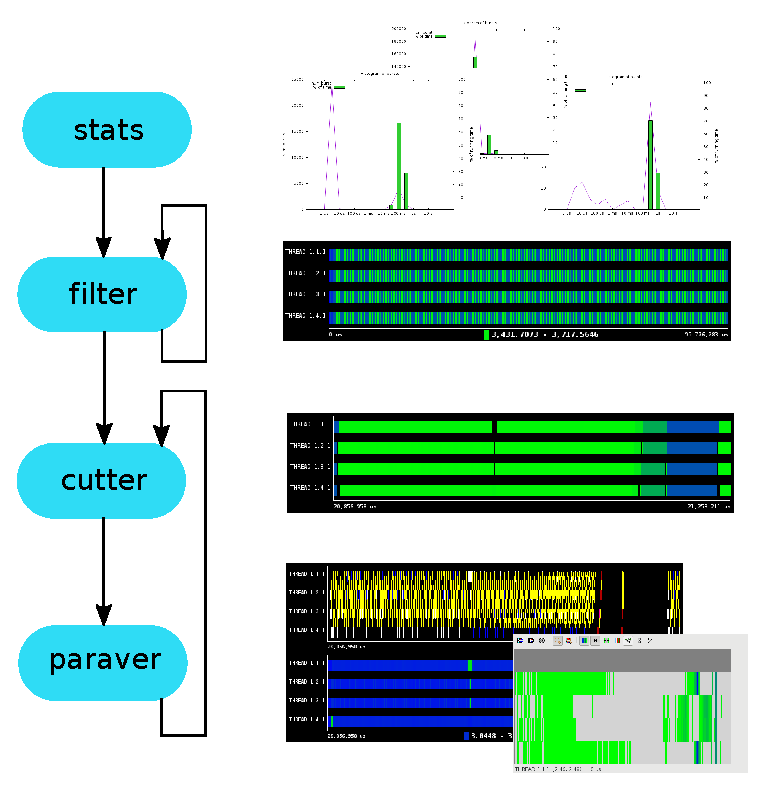
\includegraphics[width=250px]{current_analysis_flow.eps}
%\end{figure}

Talk about the BSC performance tools environment and introduce the analysis flow
with and without this proposed tool.

This is the mission of the parallel performance analysis. In an application-centric
approach, the performance analysis is a cyclic process consisting of observing 
the behaviour of the application so as to hypothesize the possible problems that 
affect its performance and finally translate these hypotheses to improvements in
the application re-starting the cycle to validate them. Obviously, the less number 
of iterations of this cycle the less time wasted and also the less money spent.


% NOTES
% .- Remember to demonstrate the interarrival time of different calls in the sam
%e loop body tend to be the same.


